\documentclass{article}

\usepackage{amsmath, graphicx}
\graphicspath{ {./images/} }

\title{Ch. 15 CW \#3 -- Solutions}
\author{Principles of Microeconomics}
\date{\today}

\begin{document}

\maketitle

\section*{Problems and Applications}

\begin{enumerate}

\setcounter{enumi}{8}
\item 

	\begin{enumerate}
	
	\item \phantom{x}

		\begin{center}
		\begin{tabular}{c | c | c | c | c}
		Q & MC& VC & TC & ATC \\
		\hline
		1 pie & \$2 & \$2 & \$11 & \$11\\
		2 & 4 & 6 & 15 & 7.5 \\
		3 & 6 & 12 & 21 & 7 \\
		4 & 8 & 20 & 29 & 7.25 \\
		5 & 10 & 30 & 39 & 7.8 \\
		6 & 12 & 42 & 51 & 8.5
		\end{tabular}
		\end{center}
	
	\item When price is \$11, the market is in equilibrium at $Q = 200$. Each producer will make 5 pies because $P$ most closely equals $MC$ when $q = 5 \text{ or } 6$. When $q = 5$, profit is
	\begin{align*}
	Profit &= (P - ATC)Q \\
	&= (11 - 7.8)(5) \\
	&= 16.
	\end{align*}
	When $q = 6$, profit is
	\begin{align*}
	Profit &= (11 - 8.5)(6) \\
	&= 15.
	\end{align*}
	Since they earn more profit when $q = 5$, they'll produce 5. 
	
	\item No, it's not because there are non-zero profits.
	
	\item In the long run, they make zero profit. Price equals the minimum of average total cost which is approximately \$7 based on part (a). Price equals the minimum of average total cost when firms are producing 3 pies each. Based on the demand schedule, 600 pies are sold in the market which means that there are $600/3 = 200$ producers.
	
	\end{enumerate}
	
\item 

	\begin{enumerate}
	
	\item \phantom{x}
	
	\begin{center}
	\begin{tabular}{c | c | c | c | c}
	Q & AVC & VC & MC & ATC \\
	\hline
	1 & \$1 & \$1 & \$1 & \$17 \\
	2 & 2 & 4 & 3 & 10 \\
	3 & 3 & 9 & 5 & 8.33 \\
	4 & 4 & 16 & 7 & 8 \\
	5 & 5 & 25 & 9 & 8.2 \\
	6 & 6 & 36 & 11 & 8.67
	\end{tabular}
	\end{center}
	
	\item Each firm produces 5 units because $P$ most closely equals $MC$ when $q = 5 \text{ or } 6$. Profit is higher when $q = 5$ (\$9 vs. \$8), so the firm produces 5 units. The total quantity supplied is $Q_S = 100q = 500$.
	
	\item Because profits are positive, firms will enter the market. As the number of suppliers increases, supply will shift right.  A rightward shift in supply drives price down and quantity demanded up. The lower price leads to a lower quantity supplied by each firm because price will equal marginal cost at a point further left on the curve. 
	
	\item Based on part (a), the minimum average total cost is approximately \$8.
	
		\begin{center}
		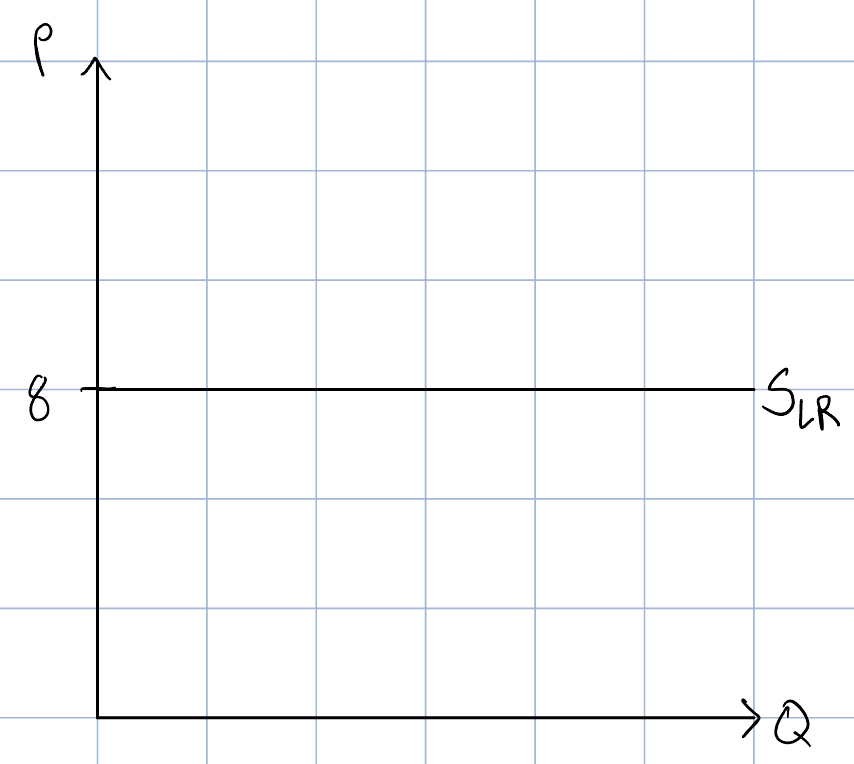
\includegraphics[width = 0.5\textwidth]{paa10c}
		\end{center}
	
	\end{enumerate}
	
\item

	\begin{enumerate}
	
	\item Fixed cost is the portion of total cost that doesn't depend on quantity, \$50. Variable cost is the part of total cost that does depend on quantity $VC = \frac{1}{2}q^2$. Average total cost is
	\begin{align*}
	ATC &= \frac{TC}{q} \\
	&= \frac{50 + \frac{1}{2}q^2}{q} \\
	&= \frac{50}{q} + \frac{1}{2}q
	\end{align*}
	
	\item You can solve this one using calculus or a graph. Alternatively, average total cost is minimized at the point where MC equals average total cost.
	
	\begin{align*}
	MC &=ATC \\
	q &= \frac{50}{q} + \frac{1}{2}q \\
	\frac{1}{2}q &= \frac{50}{q} \\
	\frac{1}{2}q^2 &= 50 \\
	q^2 &= 100 \\
	q &= 10
	\end{align*}
	
	\item The firm's supply curve is the marginal cost curve everywhere that $MC \geq ATC$. That means the firm's supply curve is 
	\begin{equation*}
	q = \begin{cases}
	P, \ P \geq 10 \\
	0, \ P < 10
	\end{cases}
	\end{equation*}
	
	\item In the short run, firm supply is the marginal cost curve everywhere that $MC \geq AVC$. $AVC = 0.5q$, so $MC \geq AVC$ for all $q \geq 0$. Therefore, market supply is \[ Q_S = 9q = 9P. \]
	
	\item \begin{align*}
	Q_S &= Q_D \\
	9P_{SR} &= 120 - P_{SR} \\
	P_{SR} &= 12 \\
	Q_{SR} &= 9(12) \\
	&= 108
	\end{align*}
	
	\item Each firm produces $q_{SR} = P_{SR} = 12$. Each firm's profit is
	
		\begin{align*}
		Profit &= TR - TC \\
		&= Pq - (50 + \frac{1}{2}q^2) \\
		&= 12(12) - (50 + \frac{1}{2}(12^2) \\
		&= 144 - 122 \\
		&= 22.
		\end{align*}
		
		Since profit is positive, firms will have an incentive to enter the market. 
		
	\item In the long run, the equilibrium price will be the minimum of ATC, so $P_{LR} = 10$. Market supply will be a horizontal line at $P_{LR} = 10$, so equilibrium quantity will be $Q_D$ when $P = 10$. That's \\ $Q_{LR} = 120 - 10 = 110$.
	
	\item In the long run, firms still produce the quantity at which $P = MC$, so $10 = q_{LR}$. That means there are $110/10 = 11$ firms in the market.
	
	\end{enumerate}

\end{enumerate}

\section*{Non-Mankiw}

\begin{enumerate}

\item 

	\begin{enumerate}
	
	\item 
	\begin{gather*}
	Q_D = 10q_D = 10(40 - 2P) = 400 - 20P \\
	Q_S = 5q_S \\
	P = \frac{q_S}{4} \implies q_S = 4P \implies Q_S = 5(4P) = 20P \\
	\end{gather*}
	
	\begin{align*}
	Q_D &= Q_S \\
	400 - 20P^* &= 20P^* \\
	400 &= 40P^* \\
	10 &= P^* \\
	Q^* &= 20(10) \\
	&= 200
	\end{align*}
	
	\[ q_S = 4P = 4(10) = 40 \]
	
	\item \[ VC = \sum_0^{40} MC = \text{Area under the MC curve} \]
	
		\begin{center}
		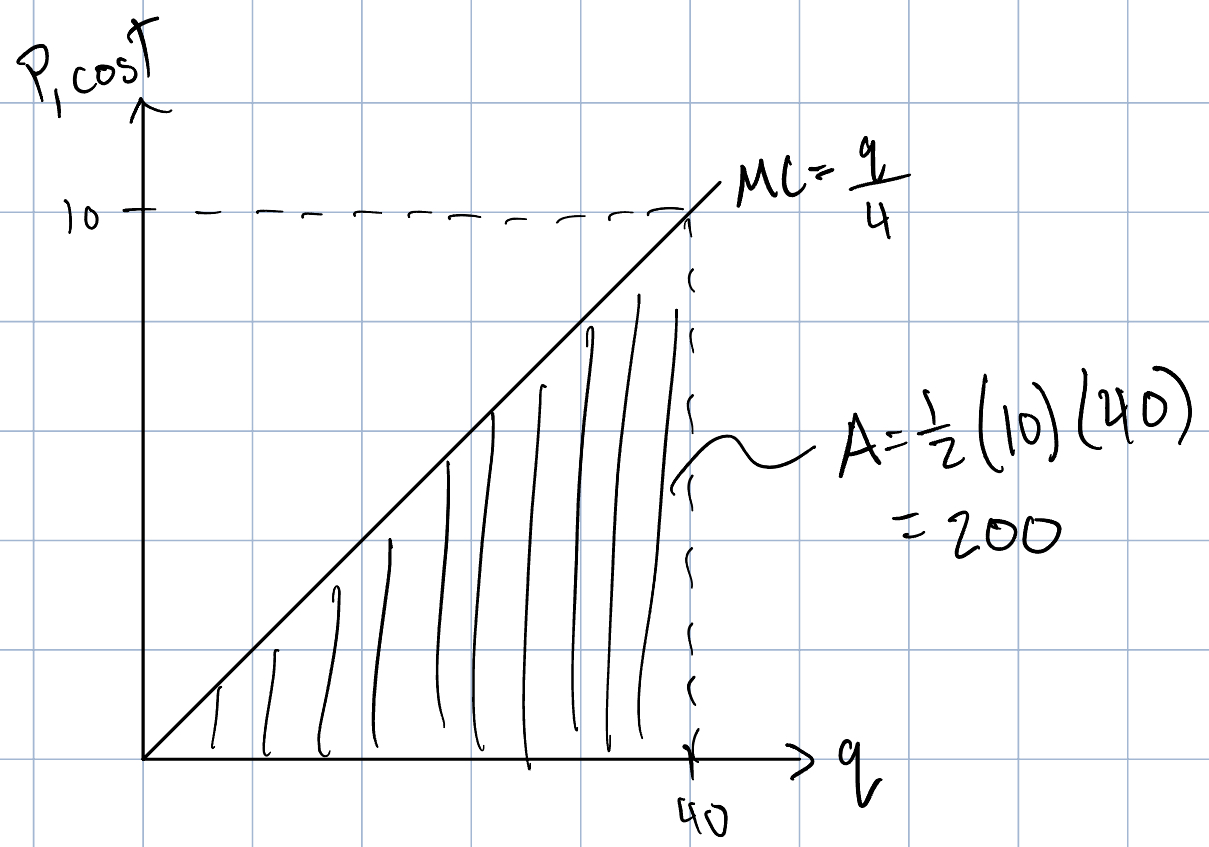
\includegraphics[width = 0.5\textwidth]{nm1b}
		\end{center}
		
	\item 
	
	\begin{align*}
	Profit &= TR - TC \\
	&= Pq - (FC + VC) \\
	&= 40(10) - (50 + 200) \\
	&= 150
	\end{align*}
	
	\end{enumerate}

\end{enumerate}

\end{document}